\lhead{\emph{State of the Art}}
\section{CHAMELEON}\label{NILM}
Although direct power meters can be replaced by indirect sensors to reduce the deployment cost~\cite{Kim09Ubicomp,Jung2010,Jung2014}, a large amount of sensors as well as technical intervention is still required. To radically decrease the implementation cost, the presence of sensors needs to be eliminated or reduced as much as possible and the state of devices needs to be determined based on the aggregate power measured at the main power supply. This approach is called Non-Intrusive Load Monitoring or NILM and firstly proposed by G.~Hart~\cite{Hart92} in the early 1990s. In recent years, there are several industrial solutions hit to the market such as Wattseeker~\cite{Wattseeker}, Smart Analyzer~\cite{smartanalyzer}. In NILM, an algorithm is developed to detect some specific features to identify the operating devices. The features are selected depending on the sampling frequency of the meters and can be classified into two classes: low frequency and high frequency.

\subsection{Architecture}\label{macro}

In the low frequency approach, the promising features relate to the real and reactive power such as average power and step-changes when switching on/off or changing the power state of a device \cite{Hart92,Drenker99}. The step-change analysis method was firstly introduced by G.Hart \cite{Hart92}, in which the large changes on the power signal, as shown in Figure~\ref{fig:A4}, are detected by an edge detector. The edge detector firstly segments the power signal into steady periods, defined as a set of consecutive instants in which the power does not vary greater than a threshold. The samples in each period are then averaged and the difference between two consecutive steady periods is called step-size. Denote $x(t)$ as the measured power at time instant $t$, $x(t)$ is then expressed as
\begin{equation}
x(t) = \sum_{i=1}^N{x_i(t)+n(t)},
\end{equation}
where $N$ is the number of devices, $x_i(t)\geq 0 $ is the power consumption of device $i$ and $n(t)$ is a noise at instant $t$. A step-change is detected if $|x(t)-x(t-1)|\geq \gamma$, with threshold $\gamma$. An event is determined as started at time $t_s$ and ended at time $t_e$ if:
\begin{equation}
\left|(x(t_s)-x(t_s-1))+(x(t_e)-x(t_e-1))\right|\leq \alpha,
\end{equation}
where $\alpha$ is a practical estimated parameter.  A cluster analysis maps the detected step-changes to a two-dimensional space of real and reactive power. The rising edge (positive step-change) and falling edge (negative step-change) of an event (device activation) are then paired together and compared with the existing clusters from the training procedure to identify the corresponding load using maximum likelihood algorithm. Figure~\ref{fig:A6} shows the position of some devices on the P-Q plane.

\begin{figure}
\centering
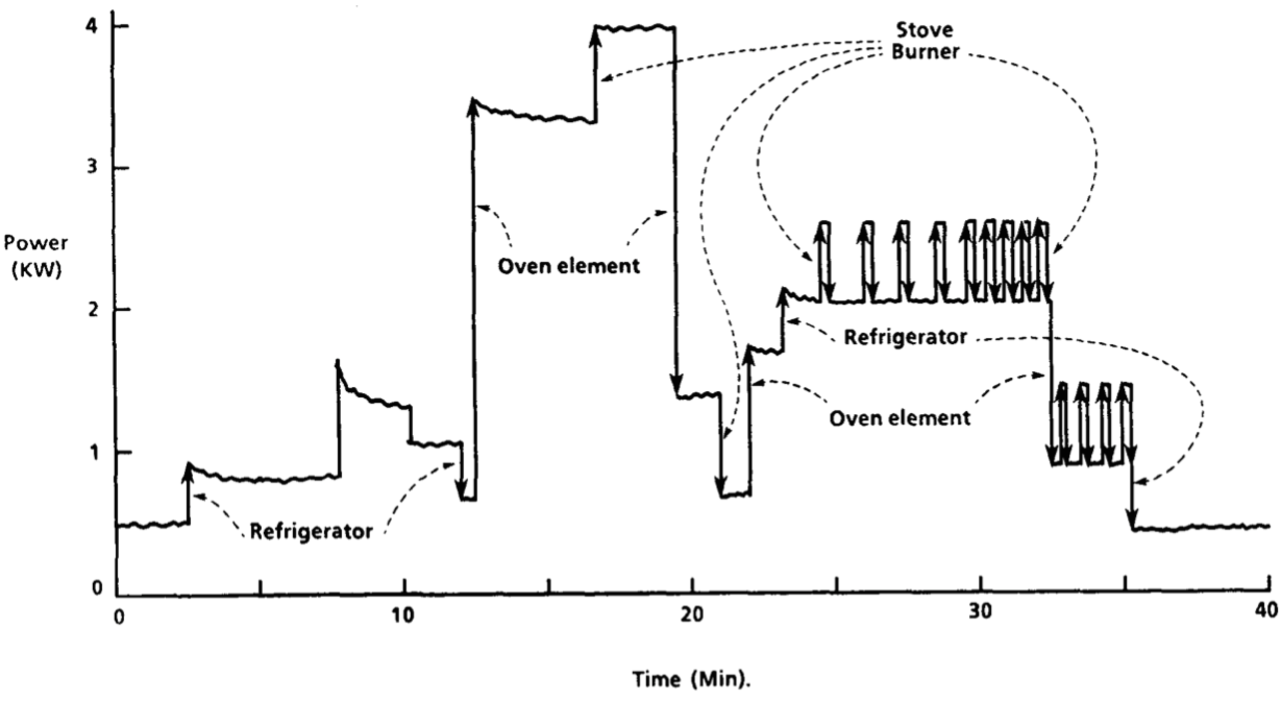
\includegraphics[width=0.8\textwidth]{./chapters/chapter2/images/step-change.pdf} 
\caption{Step-changes on the aggregate power signal~\cite{Hart92}.} 
\label{fig:A4} 
\end{figure}
%---------------------------------

The edge detector based method proposed in \cite{Hart92} is suitable to detect and identify the on/off events on the power signal. However, it cannot detect the variable loads such as computers, whose power consumption depends on the tasks. In addition, as illustrated in Figure~\ref{fig:A6}, the devices with overlapped clusters on the P-Q plane cannot be discriminated.

\begin{figure}
\centering
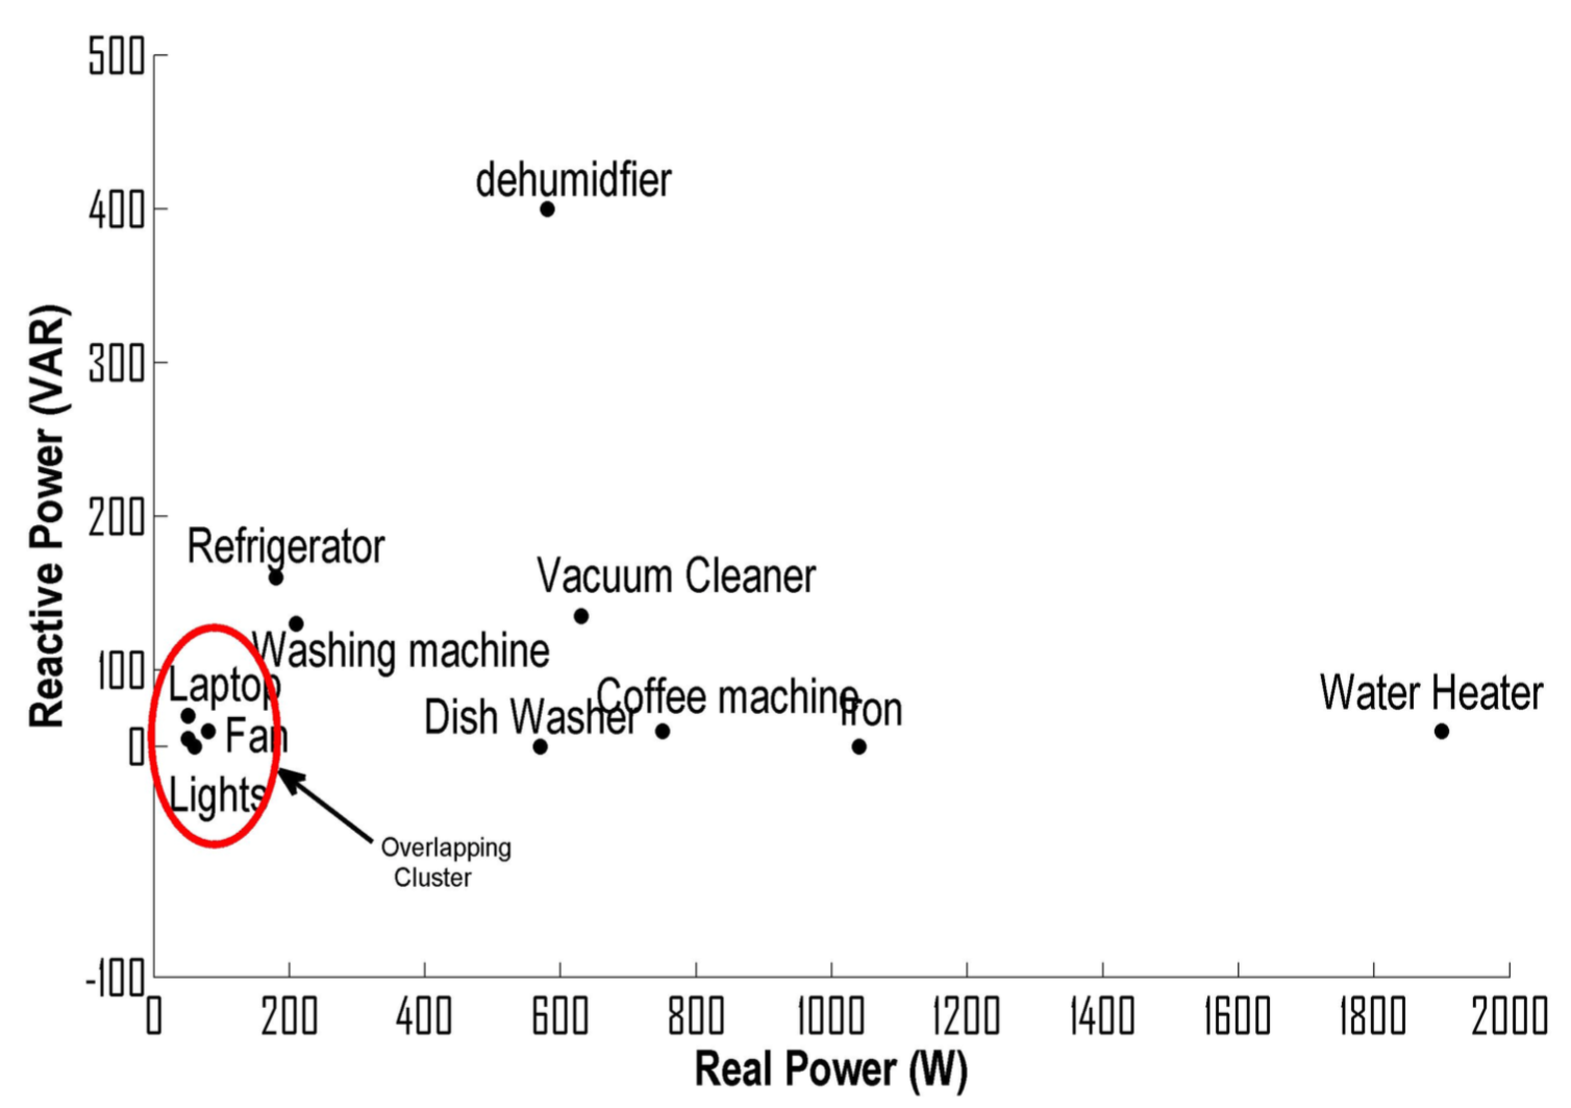
\includegraphics[width=0.8\textwidth]{./chapters/chapter2/images/overlap_PQplane.pdf} 
\caption{Load distribution in P-Q plane~\cite{Hazas11}.} 
\label{fig:A6} 
\end{figure}

To improve the performance of edge detection, some later researches are developed with some additional features. For example, in~\cite{Norford96,Marceau2000ECM}, a median filter is applied to remove the meaningless abrupt peaks in the raw signal, while in~\cite{Cole98IMTC}, edges and slopes, defined as the slow variations after an initial spike in the power signal when switching on a device, are simultaneously used as a feature to detect the devices necessary for a starting time before reaching the steady state such as heat pumps, dish washers, fridges, etc.

Similar to \cite{Hart92}, the authors of~\cite{Liao14} try to detect and pair the rising and falling edges of an event and construct a decision tree to identify the corresponding device. In the training phase, for each device, only edges with maximum and minimum height are saved instead of all possible ones. Thus, there are only $2N$ values in the library. 
The decision tree includes a\textit{ root}, several \textit{nodes} and \textit{leaves} relating to known or undefined devices. At each node, a split point value $V(node)$ calculated from the training data is used to decide the \textit{child} node, i.e. left or right. The splitting procedure iterates until any \textit{leaf} node is reached, i.e. the event is matched to a corresponding device.

Besides decision tree, another so-called Dynamic Time Warping (DTW) algorithm is also presented in~\cite{Liao14}. In this method, all active power values of an event from the rising edge to the falling edge are extracted and saved in a vector to create a pattern instead of only two edges. Because the lengths of the events are different, a pattern matching procedure via dynamic programming is proposed to apply. When a pattern is detected, the accumulated distance between it and all existing patterns in the library is calculated by Algorithm~\ref{algoA2}. The pattern giving the smallest distance is selected to identify the corresponding device. 

\begin{algorithm}[h]
\caption{Accumulated distance between two vectors with different lengths~\cite{Liao14}.}\label{algoA2}
\begin{algorithmic}[1]
\Function{DTW}{$p,q$}
	\State $n=\text{length}(p)$
	\State $m = \text{length}(q)$
	\State $D(0,0) = 0$, $D(i,0) = D(0,i)=\infty$
	\For {$i=1,\ldots,n$}
		\For {$j=1,\ldots,m$}
			\State $d(i,j)=|p(i)-q(j)|$
			\State $D(i,j) = d(i,j)+\min{\{D(i-1,j),D(i-1,j-1),D(i,j-1)\}}$
		\EndFor
		\State \textbf{end for}
	\EndFor
	\State \textbf{end for}
	\State Output $D(n,m)$
\EndFunction
\State \textbf{end function}
\end{algorithmic}
\end{algorithm}
The simulation results with REDD dataset~\cite{Liao14}, as shown in Table~\ref{TA1}, point out that the DTW algorithm outperforms the Hidden Markov Model (HMM) approach \footnote{presented later in this chapter} in terms of detection reliability as well as sensibility to the events. 
\begin{table}
\caption{Performance comparison between DTW and HMM approaches~\cite{Liao14}.}\label{TA1}
\begin{center}
\begin{tabular}{|c|c|c|c|c|}
\hline
 &\multicolumn{2}{|c|}{Reliability (\%)}  &  \multicolumn{2}{|c|}{Sensibility (\%)} \\ \hline
 House & DTW  & HMM & DTW  & HMM  \\ \hline
 House 1 & 85.01  & 79.29 & 79.72 & 62.72  \\ \hline 
 House 2 & 89.86  & 51.80 & 84.39  & 62.79  \\ \hline
 House 6 & 98.86  & 99.30 & 81.22  & 74.74  \\ \hline
\end{tabular}
\end{center}
\end{table}

The active power values can also be used to compute the load distribution~\cite{Chuang11}. Whenever an event is detected on the aggregate power signal, the corresponding load distribution will be calculated and compared with the library to identify the device. To get the load distribution when two or more devices operate at the same time, the convolution is applied to the distribution of the corresponding devices.
Meanwhile, the authors of \cite{Batra2013} apply the edge detector to each phase of electric power supply. This division helps to reduce the state space from $K^N$ down to $K^{N_p}$ if each device has $K$ states and each phase supplies the power for $N_p$ devices. Obviously, this method is efficient when applied in large buildings with more than one phase of electric power.

In another research, to identify large loads such as water heaters, the authors of~\cite{Farinaccio99EB} propose a so-called \textit{top-bottom rule-based} algorithm comprised of many decision rules applied to each detected pattern such as step-change, average power, total power, number of data points, etc. After comparing each component with the library, a final score is calculated to make a final decision about the operation of the corresponding device. Each type of devices is recognized by a different set of rules, which implies that this method need an excessive training and makes it difficult to be widely implemented.

Instead of detecting the events on the aggregate power signal, the raw power data can also be directly used in sparse coding~\cite{Kolter10,Pathak15}. In this method, the training data of each device is contained in matrix $\mathbf{W}_i\in \mathbb{R}^{T\times m}$ in which each column corresponds to the data of one week. The aggregate power consumption is then $\mathbf{W}=\sum_{i=1}^N{\mathbf{W}_i}$. Applying the sparse coding, the following approximation is considered: 
\begin{equation}
\mathbf{W}_i=\mathbf{B}_i\times \mathbf{A}_i, 
\end{equation}
where $\mathbf{B}_i\in \mathbb{R}^{T\times n}$ contains $n$ basis functions or \textit{dictionary}, and $\mathbf{A}_i\in \mathbb{R}^{n\times m}$ contains the \textit{activations} of basis functions. In the training period, the values of $\mathbf{B}_i$ and $\mathbf{A}_i$ are estimated by the following minimization:
\begin{equation}
\smash{\displaystyle\min_{\mathbf{A}_i\geq 0,\mathbf{B}_i\geq 0}{\frac{1}{2}\parallel \mathbf{W}_i-\mathbf{B}_i\times \mathbf{A}_i\parallel_F^2 + \lambda\sum_{p,q}{(\mathbf{A}_i)_{pq}}}} \mbox{ subject to } \parallel b_i^{(j)} \parallel_2 \leq 1, j=1,\ldots,n,
\end{equation}
where $\parallel \mathbf{Y}\parallel_F \equiv (\sum_{p,q}{\mathbf{Y}_{pq}})^{1/2}$ denotes the Frobenius norm, and $\parallel y \parallel_2 \equiv (\sum_{p}{y_p^2})^{1/2}$ is the $l_2$-norm.
To disaggregate a new set of data $\mathbf{X}\in \mathbb{R}^{T\times m'}$, the value of $\mathbf{A}_i$ is recalculated as
\begin{equation}
\begin{split}
\hat{\mathbf{A}}_{1:N}=&\argmin_{\mathbf{A}_{1:N}\geq 0}{\parallel \mathbf{X}-\left[ \mathbf{B}_1\cdots \mathbf{B}_N\right] \left[\begin{array}{c}\mathbf{A}_1\\ \vdots \\ \mathbf{A}_N \end{array}\right]  \parallel_F^2 + \lambda \sum_{i,p,q}{(\mathbf{A}_i)_{pq}}}\\
&\equiv \argmin_{\mathbf{A}_{1:N}\geq 0}{F(\mathbf{X},\mathbf{B}_{1:N},\mathbf{A}_{1:N})}.
\end{split}
\end{equation}
Finally, the power is disaggregated to each device by
\begin{equation}
\hat{\mathbf{X}}_i=\mathbf{B}_i\times \hat{\mathbf{A}}_i.
\end{equation}
Obviously, the sparse coding based disaggregation algorithm needs an excessive amount of training data. Additionally, this method is only used in off-line mode and not suitable for the real-time detection.


To recognize the large loads as in \cite{Farinaccio99EB}, Prudenzi~\cite{Prudenzi02} applies Artificial Neural Networks (ANN) to determine the time of use of three different loads from two groups including water heater (group H) and washing machine/dish washer (group W), as illustrated in Figure~\ref{fig:A10}. In the preprocessing stage, the daily data is sampled every 15 minutes and segmented into six 8-hour patterns with 4-hour overlapped interval. Then, to classify these patterns into two clusters with and without power activation (cluster P and cluster A, respectively), three parameters including maximum power, average power and maximum power change in each pattern are applied to a Self-Organizing Map (SOM). The patterns in cluster P are then sent to the identification stage comprising two supervised Back-Propagation neural Networks (BPN) with 32 inputs, 24 hidden neurons and 32 outputs. The first net (BPN1) tries to detect the instants with energy usage in each pattern and fills in a $6\times 32$-cell output table. After that, the output is filtered by multiplying by the output of the preprocessing stage and sent to the second net (BPN2), where the patterns of group H will be discriminated from group W by applying the moving average operation. The output of this net will only contain the power usage indicators of the water heater. Combining the outputs of two neuron nets, the time of use of both groups will be determined in the post-processing stage. Although this research only considered two groups of devices, it contributes a new promising approach for pattern identification by applying ANN.

\begin{figure}
\centering
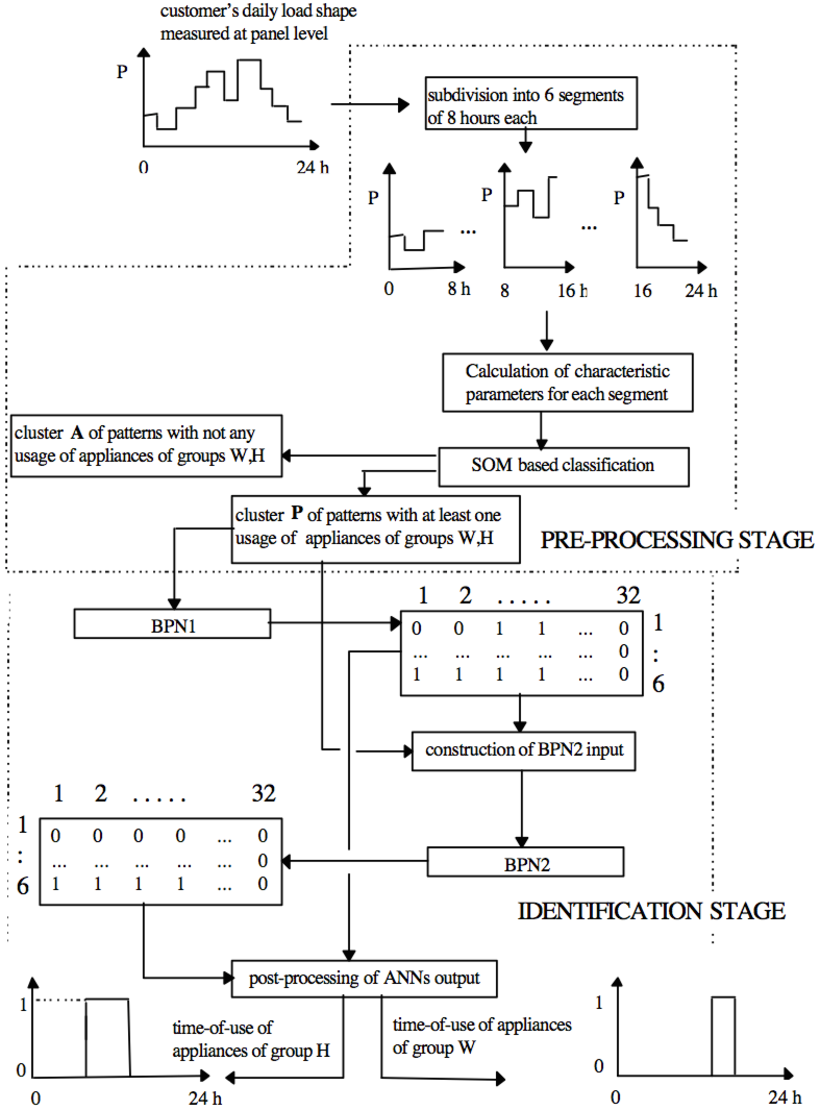
\includegraphics[width=0.6\textwidth]{./chapters/chapter2/images/3-stage_ANN.pdf} 
\caption{ANN to identify the water heater (group H) and washing machine/dish washer (group W)~\cite{Prudenzi02}.} 
\label{fig:A10} 
\end{figure}

Similarly, an ANN architecture is also applied in a system called real-time RECognition of electrical Appliances and Profiling (RECAP)~\cite{Ruzzelli10,Najmeddine08,Figueiredo11}, where the current and voltage waveforms are analyzed to extract the peak and Root Mean Square (RMS) values of both current and voltage, phase difference and power factor to define a profile of device. Besides, two other factors including signature length and sampling frequency are also captured to standardize the signatures from dissimilar types of energy meters. Although the RECAP system can profile and recognize the devices under a single framework and show a good performance when identifying the kitchen devices, it is not suitable for the multi-state devices.


% Add: Neural NILM

In another research, deep neural networks are constructed to disaggregate the domestic energy \cite{KellyK15} and applied to the UK Domestic Appliance-Level Electricity (UK-DALE) dataset \cite{UK-DALE}. The input of the network is a window of aggregate data with length determined by the maximum operating duration of the target device, while the output contains the information to reconstruct its power consumption. Before to be fed to the network, the input sequence in each data window is normalized by subtracting by the mean of sequence and by dividing by the standard deviation. The device activations used as the targets in training the networks are extracted based on some arguments such as maximum power, on-power threshold, minimum on-duration, minimum off-duration~\cite{Batra14}. The authors of \cite{KellyK15} propose three deep learning architectures to reconstruct the power consumption of target devices. The first one is a Recurrent Neural Network (RNN), which allows the output from each neuron in a layer at time step $t$ to be fed via weighted connections to all neurons of that layer at time step $(t+1)$. This makes RNNs suitable for the sequential data. To enhance the performance of RNNs in term of memory, the Long Short-Term Memory (LSTM) architecture \cite{Hochreiter97}, using the memory cells with a gated input, gated output and gated feedback loop, is applied. Besides, a bidirectional RNN, which is composed of two parallel RNNs, one for the input sequence forwards and one for the input sequence backwards, is also applied. The concrete architecture with type of each layer is as follows: Input $\rightarrow$ CONVolutional layer (CONV) $\rightarrow$ Bidirectional RNN layer (BiRNN) $\rightarrow$ BiRNN $\rightarrow$ Fully Connected layer (FC) $\rightarrow$ FC (Output). Examples of neural networks using CONV, BiRNN and FC are given in Figure~\ref{fig:AA3}.


The second deep learning architecture is Denoising Autoencoder (DAE) \cite{Vincent08}. The role of this architecture is to recover the power consumption of the target devices from the background noise. To do that, the DAEs at first try to encode the input to a compact vector with a coding layer and then decode it to reconstruct the input. The proposed architecture of DAEs includes six layers, in which the first convolutional layer can be considered as an encoder and the last one is a decoder, as follows: Input $\rightarrow$ CONV $\rightarrow$ FC $\rightarrow$ FC $\rightarrow$ FC $\rightarrow$ CONV (Output).


Meanwhile, in the last architecture, the power activation in each data window can be reconstructed by detecting the  start time, end time and average power consumption. In other words, they want to draw a rectangle around each activation in which the left side is the start time, right side is the end time and the height is the average power. Therefore, the output layer of this network includes three neurons and the output data are encoded to be in the range $[0,1]$. The exact architecture consists of eight layers: Input $\rightarrow$ CONV $\rightarrow$ CONV $\rightarrow$ FC $\rightarrow$ FC $\rightarrow$ FC $\rightarrow$ FC $\rightarrow$ FC (Output).
\begin{figure}[htb]
\begin{minipage}[h]{1\linewidth}
\centering
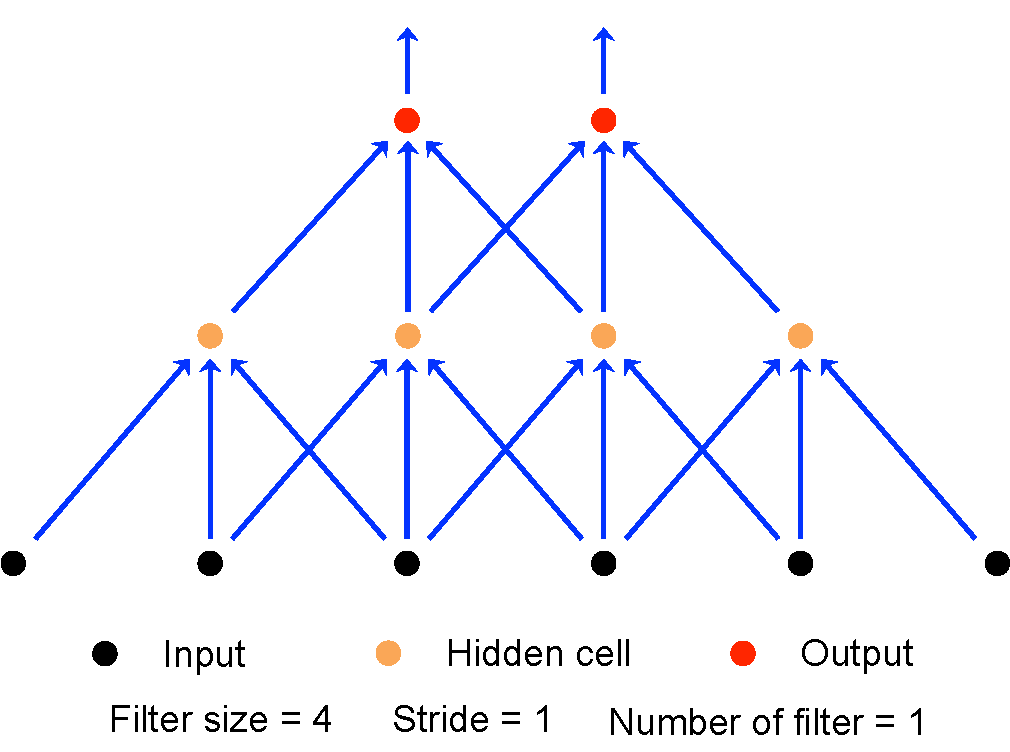
\includegraphics[width=0.48\textwidth]{./chapters/chapter2/images/ConvANN.pdf}
%  \vspace{1.5cm}
\centerline{(a) Convolutional neural network}\medskip
\end{minipage}
\hfill
\begin{minipage}[h]{1\linewidth}
\centering
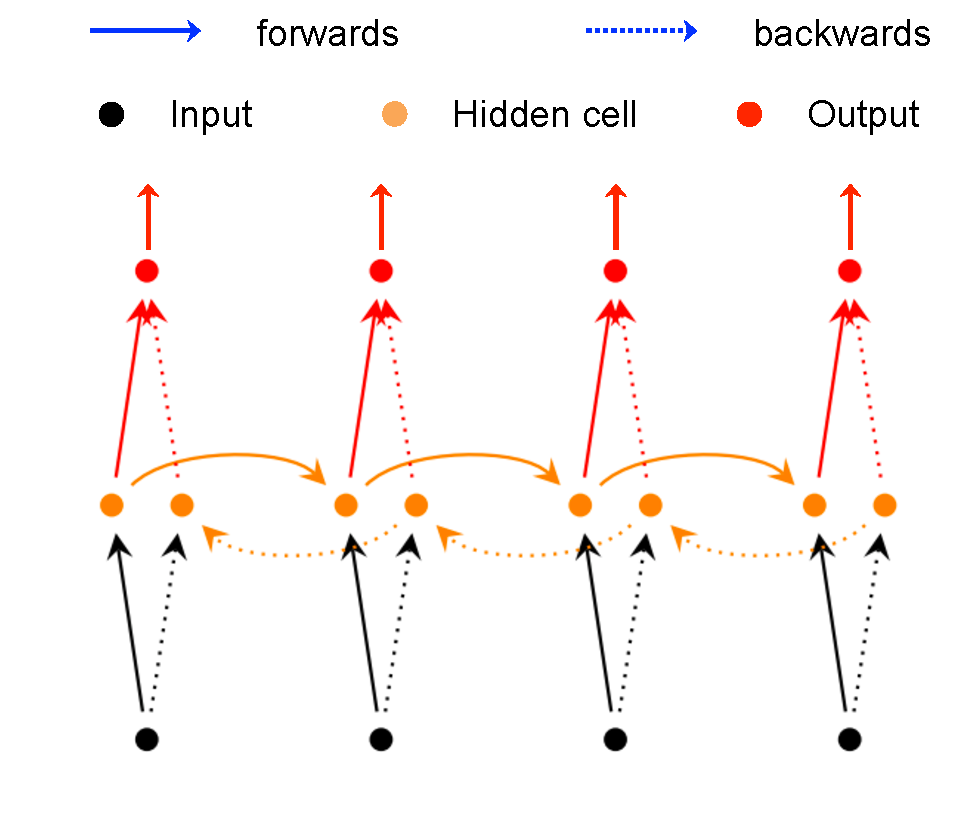
\includegraphics[width=0.48\textwidth]{./chapters/chapter2/images/BiRNN.pdf}
%  \vspace{1.5cm}
\centerline{(b) Bidirectional RNN}\medskip
\end{minipage}
\hfill
\begin{minipage}[h]{1\linewidth}
\centering
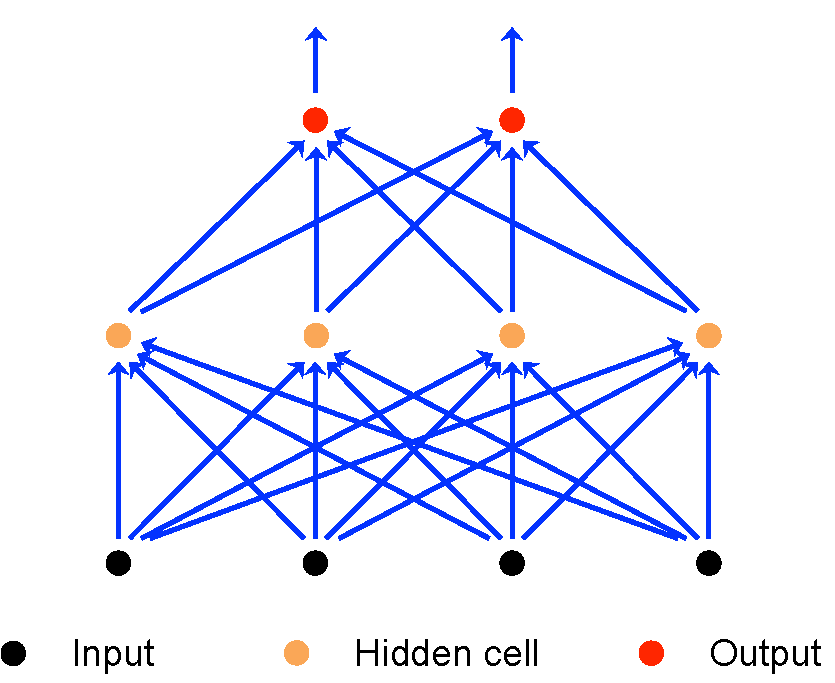
\includegraphics[width=0.48\textwidth]{./chapters/chapter2/images/fullyConn.pdf}
%  \vspace{1.5}
\centerline{(c) Fully connected neural network}\medskip
\end{minipage}
\caption{Examples of convolutional neural network, bidirectional RNN and fully connected neural network.}
\label{fig:AA3}
%
\end{figure}

Figure~\ref{fig:AA4} illustrates the outputs produced by three deep neural networks in~\cite{KellyK15}. Apparently, the DAE architecture performs a good estimation for the varying power consumers such as washing machine, while the third architecture (Rectangles) is suitable for the stable loads such as kettle, fridge. In addition, the RNN using LSTM architecture gives a worse estimation than DAE but better than Rectangles with variable loads.

\begin{figure}
\centering
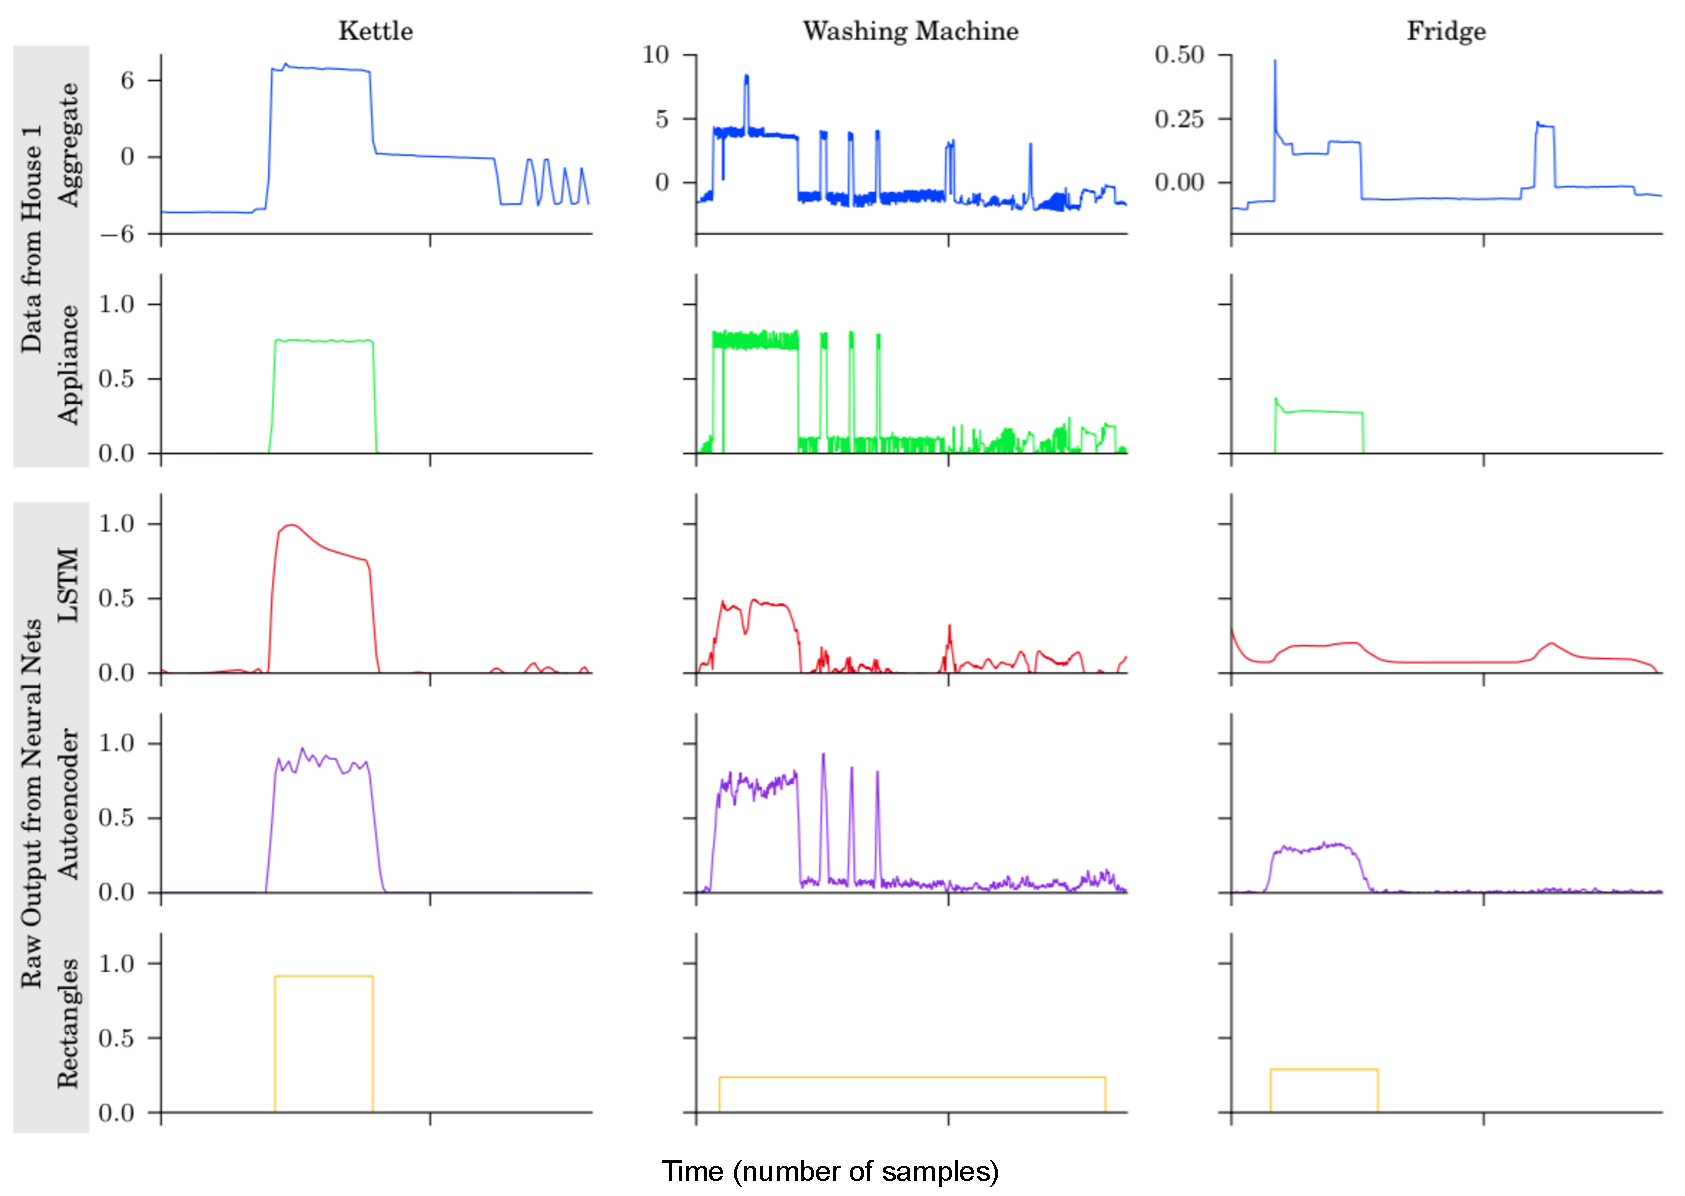
\includegraphics[width=1\textwidth]{./chapters/chapter2/images/neuralNILM.pdf} 
\caption{Outputs produced by three deep neural networks~\cite{KellyK15}.} 
\label{fig:AA4} 
\end{figure}

Besides ANN, HMM is also applied to find the state of devices in NILM~\cite{Parson12,Kim11ICDM,Kolter11redd,Nambi13,Lukaszewski13,Zoha13,Jia15,Ridi14}. The state of each device can be considered as a hidden variable, while the observations relate to the aggregate power consumption. In~\cite{Parson12}, the aggregate power consumption $x$ as well as the difference on the power between two consecutive time slices, denoted as $y=x_i-x_{i-1}$, are considered as the observations of a so-called difference HMM, as represented in Figure~\ref{fig:A11}, to find the state sequence $s$ of the devices.
\begin{figure}
\centering
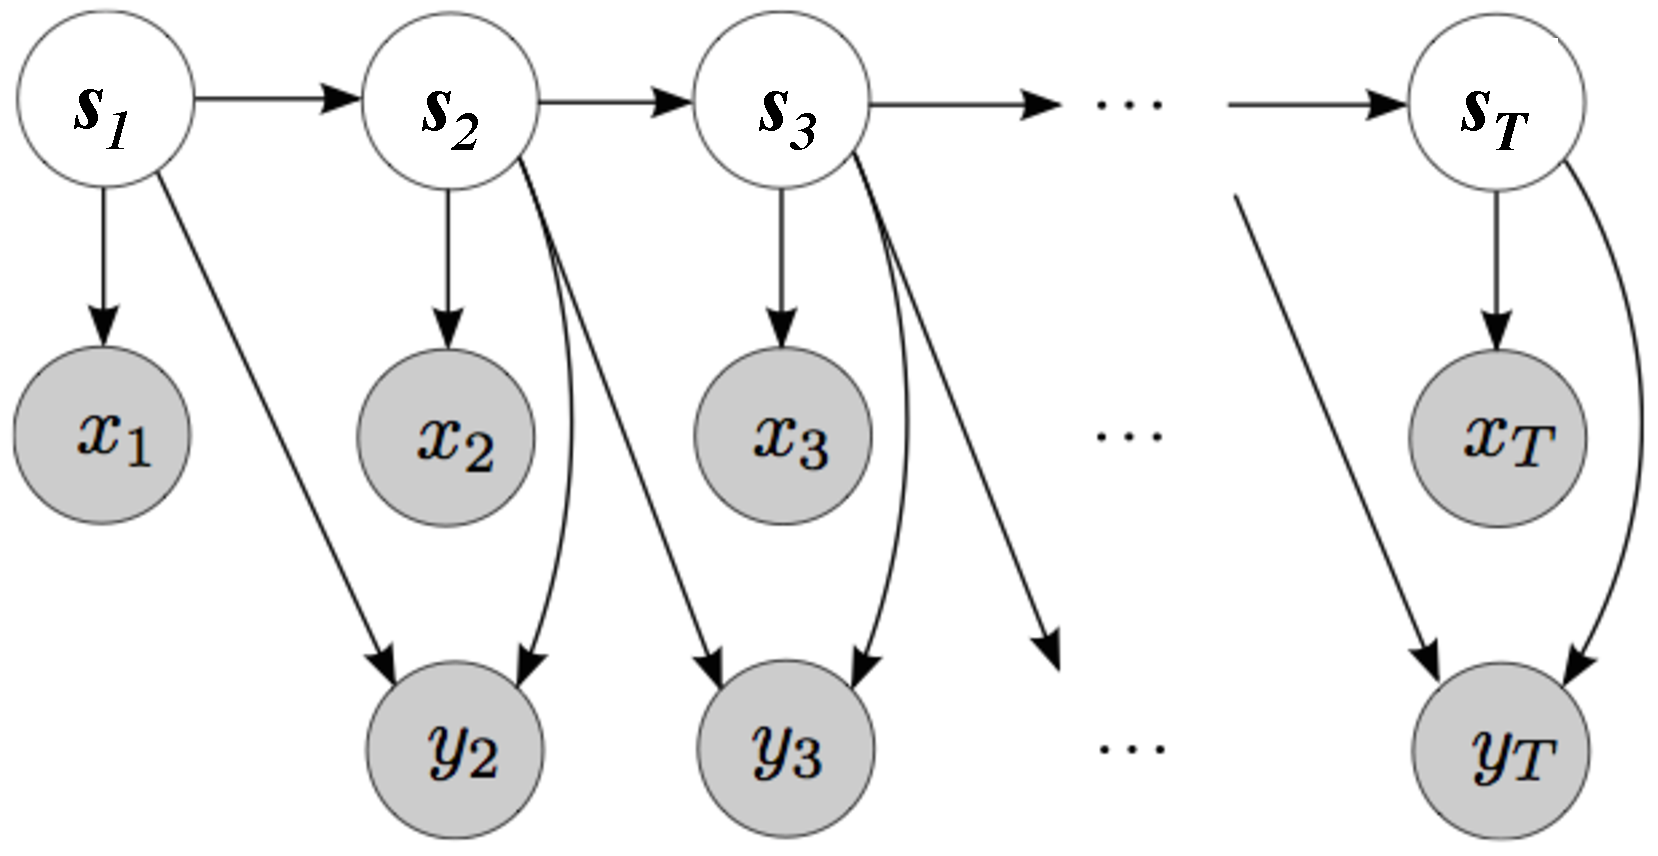
\includegraphics[width=0.5\textwidth]{./chapters/chapter2/images/HMM.pdf} 
\caption{Difference HMM~\cite{Parson12}. Shaded nodes represent the observations and unshaded nodes represent the hidden variables.} 
\label{fig:A11} 
\end{figure}
The correlation of the variables in this model are defined by a set $\theta$ of three parameters learned from the training dataset 
\begin{equation}
\theta = \{\pi ,\mathbf{A},\phi\},
\end{equation}
where $\pi$ denotes the probability of the initial state, $\mathbf{A}$ the transition probability matrix from a state at time $(t-1)$ to another at time $t$ and $\phi$ the emission probability generated by a state and assumed to follow the Gaussian distribution. Besides, a constraint that a device is only in on-state if the aggregate power is larger than its own power demand is also necessary to be imposed.
The state of each device is determined by applying the extension of Viterbi algorithm through two steps. In the first step, a filter is applied to suppress the observations whose joint probability does not excess the predefined threshold and the second step evaluates the joint probability of all sequences $x$, $y$, $s$ to identify the state of devices is defined as
\begin{equation}
\begin{split}
p(x,y,s|\theta)=p(s_1|\pi)\prod_{t=2}^{T}{p(s_t|s_{t-1},\mathbf{A})}
\prod_{t=1}^{T}{P(w_{s_t}\leq x_t|s_t,\phi)}\prod_{t\in S}{p(y_t|s_t,s_{t-1},\phi)},
\end{split}
\end{equation}
where $S$ is the set of filtered observations and $T$ is the length of observation sequence.

Meanwhile, in~\cite{Kim11ICDM}, only the aggregate power consumption is considered as observation sequence. In this research, the on-duration of home devices can be modeled as following the gamma distribution with a couple of parameters $\kappa^{(i)}$, $\theta^{(i)}$ for each device $i$. This assumption is drawn from the on-duration histogram of some popular electrical devices such as television, laptop, monitor, etc. as shown in Figure~\ref{fig:AA12}. Moreover, some additional features such as time of day, day of week and environment information from a monitoring sensors network are also taken into account. Considering $K$ additional conditions with corresponding sequences $c^{(1)}, \ldots, c^{(K)}$ in HMM creates a Conditional Factorial Hidden Semi-Markov Model (CFHSMM) and is illustrated by the graphical model in Figure~\ref{fig:A12}. 

\begin{figure}
\centering
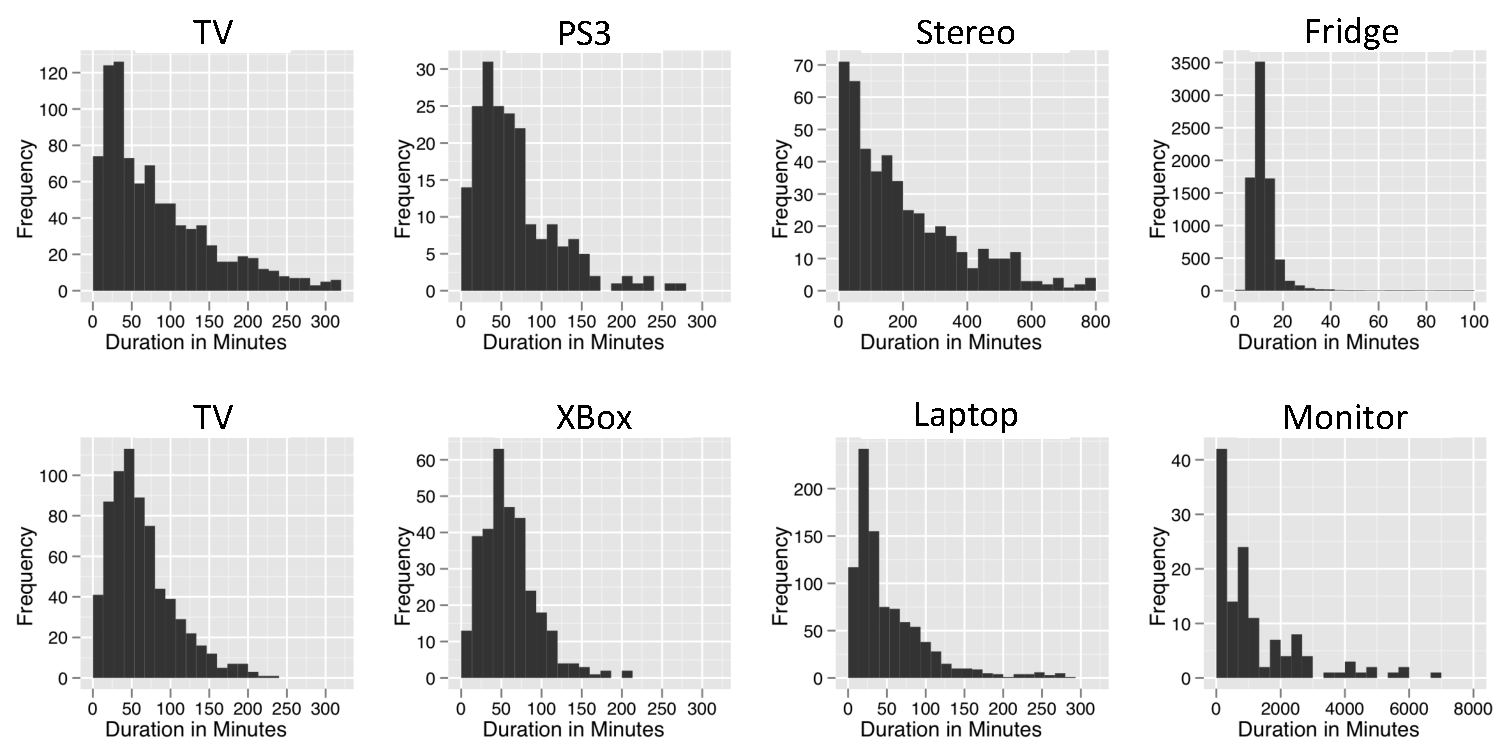
\includegraphics[width=1\textwidth]{./chapters/chapter2/images/on-duration_gamma.pdf} 
\caption{On-duration histogram of some devices~\cite{Kim11ICDM}.} 
\label{fig:AA12} 
\end{figure}

\begin{figure}
\centering
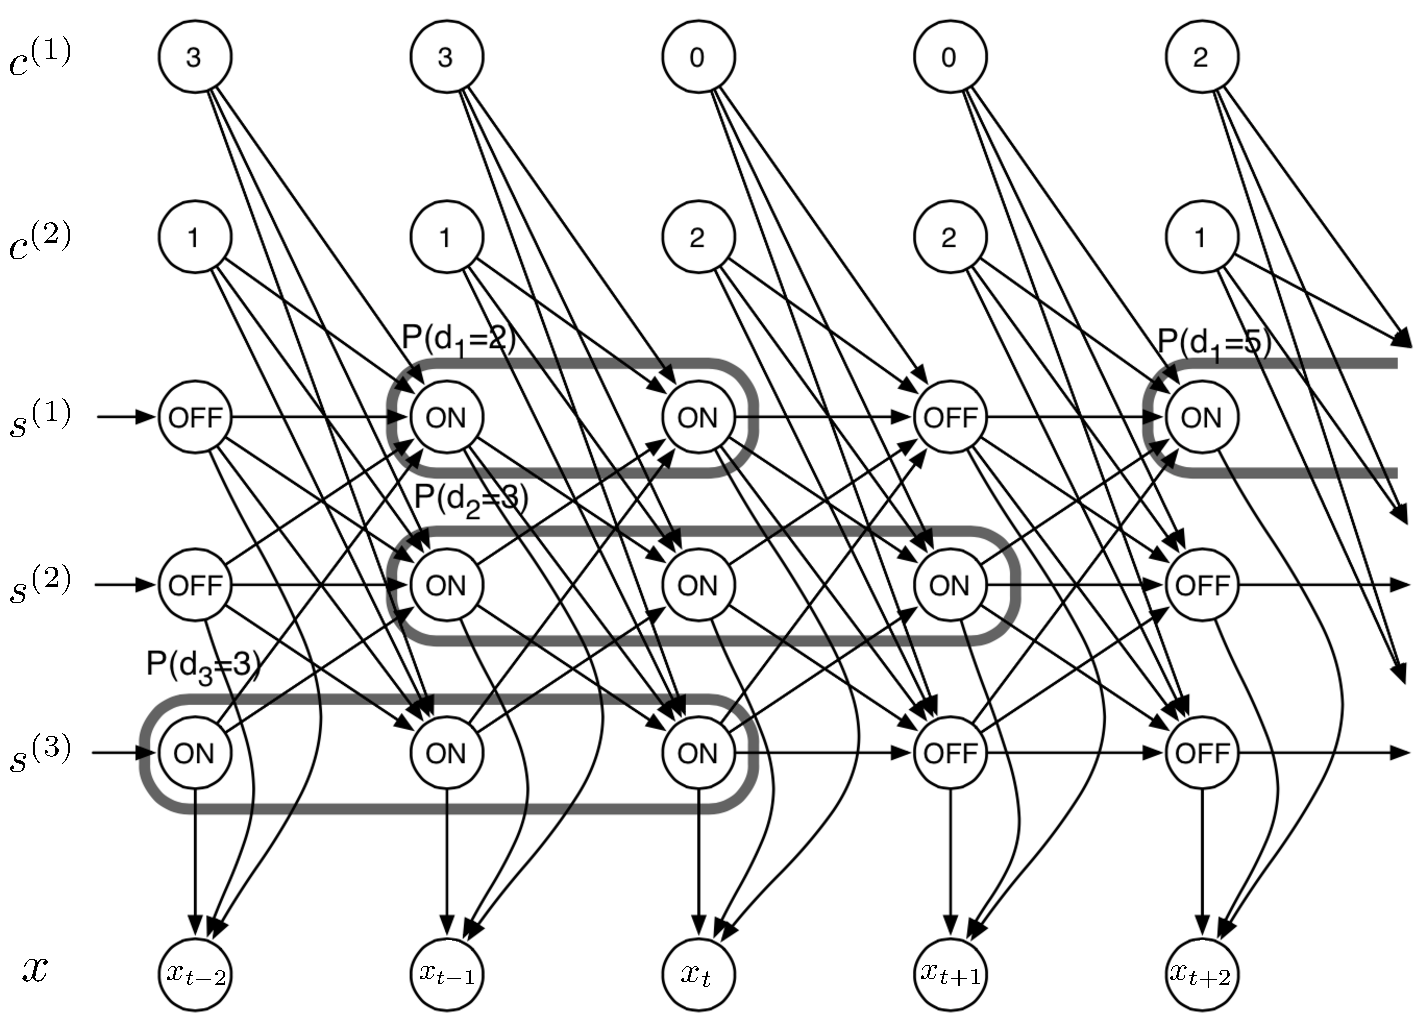
\includegraphics[width=.8\textwidth]{./chapters/chapter2/images/CFHSMM.pdf} 
\caption{Graphical representation of CFHSMM with the additional conditions $c^{(1)}$, $c^{(2)}$~\cite{Kim11ICDM}.} 
\label{fig:A12} 
\end{figure}

The hidden variables $s^*$ of this model can be found by applying the Maximum Likelihood Estimation (MLE) after training the set of parameters $\lambda$,
\begin{equation}
s^*=\argmax_{s}{P(X,s|\lambda)},
\end{equation}
where $P(X,s|\lambda)$ is the joint probability computed by the product of the initial probability $\psi_{in}(X,s|\lambda)$, the emission probability $\psi_e(X,s|\lambda)$, and the transition probability $\psi_t(X,s|\lambda)$, i.e.,
\begin{equation}
P(X,s|\lambda)=\psi_{in}(X,s|\lambda)\times \psi_e(X,s|\lambda)\times \psi_t(X,s|\lambda).
\end{equation}
The difference of this model compared to other HMMs is the consideration of external information in estimating the transition probability, as follows:
\begin{equation}
\begin{split}
\psi_t(X,s|\lambda)=&\prod_{i=1}^{N}{\prod_{t:s_t^{(i)}=0}{\left(\left(\prod_{j=1}^N{m_{s_{t+1}^{(i)}js_t^{(j)}}^{(i)}} \right) \left(\prod_{j=1}^K{f_{s_{t+1}^{(i)}jc_t^{(j)}}^{(i)}}\right)\right)}}\\
&\prod_{t:s_t^{(i)}=1}{\left(\left(\prod_{j=1:i\neq j}^N{m_{s_{t+1}^{(i)}js_t^{(j)}}^{(i)}} \right)\left(\prod_{j=1}^K{f_{s_{t+1}^{(i)}jc_t^{(j)}}^{(i)}}\right)\right)}\\
&\prod_{t:s_t^{(i)}=1,s_{t-1}^{(i)}=0}P(d=l_t^{(i)}|\kappa^{(i)},\theta^{(i)}),
\end{split}
\end{equation}
where $m_{kjl}^{(i)} = P(s_{t}^{(i)}=k|s_{t-1}^{(j)}=l)$ is the conditional probability for device $j$ of state $l$, $f_{kjl}^{(i)} = P(s_{t}^{(i)}=k|c_{t-1}^{(j)}=l)$ is the conditional probability for external feature $j$ of value $l$, $d$ is the on-duration length and $l_t^{(i)}$ is the length of on-duration of device $i$ beginning from time $t$.

Another less complex model of CFHSMM also applied in NILM is the Factorial Hidden Markov Model (FHMM) \cite{Kolter11redd,Nambi13,Lukaszewski13,Zoha13,Jia15}, in which the states of each device are considered as a hidden sequence and the external information is ignored. In those researches, we can find a Nonparametric Factorial Hidden Markov Model~\cite{Jia15}, which helps to eliminate the need of sub-metered data to train the model or the prior knowledge about the number of devices. Nevertheless, detecting the devices with many levels of power demand is a challenge. Constructing the problem in the context of NILM as an HMM can give an effective state determination approach for low-frequency power measurement. It helps to improve the accuracy and opens many perspectives to develop in future work. The accuracy of this method varies depending on the type and number of devices. Nevertheless, this approach has some limitations such as excessive training period to consider the distribution of the variables as well as complexity computation.







\subsection{Optical Network Interface}\label{micro}

In many cases, low-frequency based algorithms cannot discern the devices with the same power characteristics such as power demand, operating duration, rising and falling edges, etc. Besides, if a device consumes a variable energy over time, the steady state does not exist and the detection algorithm cannot accurately execute. Therefore, studies on other algorithms based on a higher sampling frequency are necessary. These algorithms will focus on harmonics and especially transient phase, which contains much useful information about the devices.

\begin{figure}[!ht]
\centering
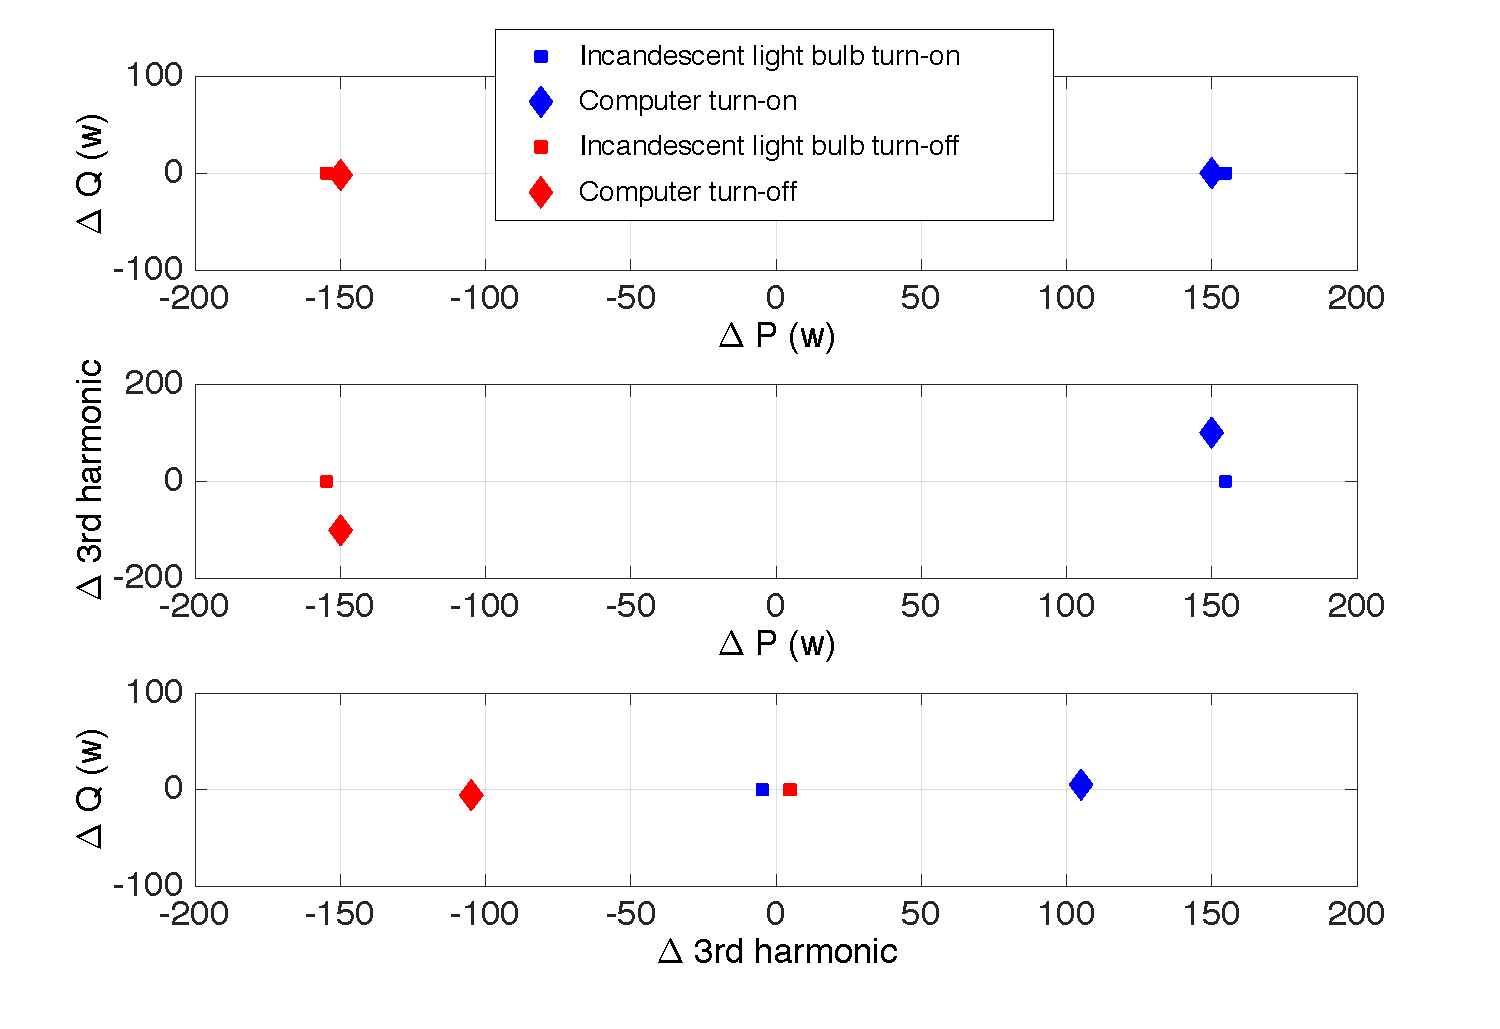
\includegraphics[width=0.8\textwidth]{./chapters/chapter2/images/third_harmonic_discrimination.pdf} 
\caption{A computer and an incandescent light bulb cannot be discriminated by the real and reactive power but can be distinguished by analyzing the third harmonic~\cite{Laughman03PEM}.} 
\label{fig:A14} 
\end{figure}
In \cite{Liang10I,Liang10II,Laughman03PEM,Cole2000,Suzuki08,Li12}, the authors propose to use the Fourier transform to determine the current harmonics. In~\cite{Laughman03PEM}, the indistinguishable problem of the devices consuming the same power in~\cite{Hart92} is solved by using the third harmonic obtained from the phase-locked short-time Fourier transform of current waveform collected at 8000~Hz and higher sampling frequency. As shown in Figure~\ref{fig:A14}, an incandescent light bulb and a computer cannot be discriminated by the first harmonics, i.e. real and reactive power, but can be distinguished by analyzing the third harmonics. Additionally, as presented in~\cite{Laughman03PEM}, the operating devices can also be detected by matching the events on the transient phase with the predefined signatures obtained from the training period. For example, the transient phases of a computer and an incandescent lamp are distinguishable because heating a lamp filament is different from charging the power supply or the batteries of a computer. Furthermore, transient-based recognition also allows near-real-time identification of energy consumers.
That is the reason why the transient signal is studied in many other researches \cite{Shaw08,Cox06,Yang07,Lin10,Chang11, Leeb95PD,Chang08,Lee05,Wichakool09,Chang12}.

In \cite{Shaw08,Cox06}, short-time Fourier transform is used to compute the spectral envelope coefficients of the transient signal when starting a device. The electrical load transients detected by the system will be classified by comparing with the existing transient signatures in the library.
In contrast, the authors of \cite{Yang07,Lin10,Chang11} try to apply an ANN to process the transient signal. In \cite{Yang07}, the transient period is segmented into windows and a wavelet transform is applied to each one. Meanwhile, the load current acquisition can be measured instead of power consumption to reduce the complexity and computation~\cite{Lin10}. ANN can also be combined with a genetic algorithm to identify load demands and improve recognition accuracy of NILM results~\cite{Chang11}. 

However, detecting complete transient shapes is sometimes a waste of memory and not necessary. That is the reason why in~\cite{Leeb95PD}, the authors introduce a new time pattern called \textit{v-shape}, which is the periods containing the significant changes during the transient phase. Figure~\ref{fig:A15} shows an example of the \textit{v-shapes} in the transient signal of an induction motor. The principle of \textit{v-shape}-based identification is to search for the precise time pattern of \textit{v-shape} and compare with the existing patterns in the library.
\begin{figure}[!ht]
\centering
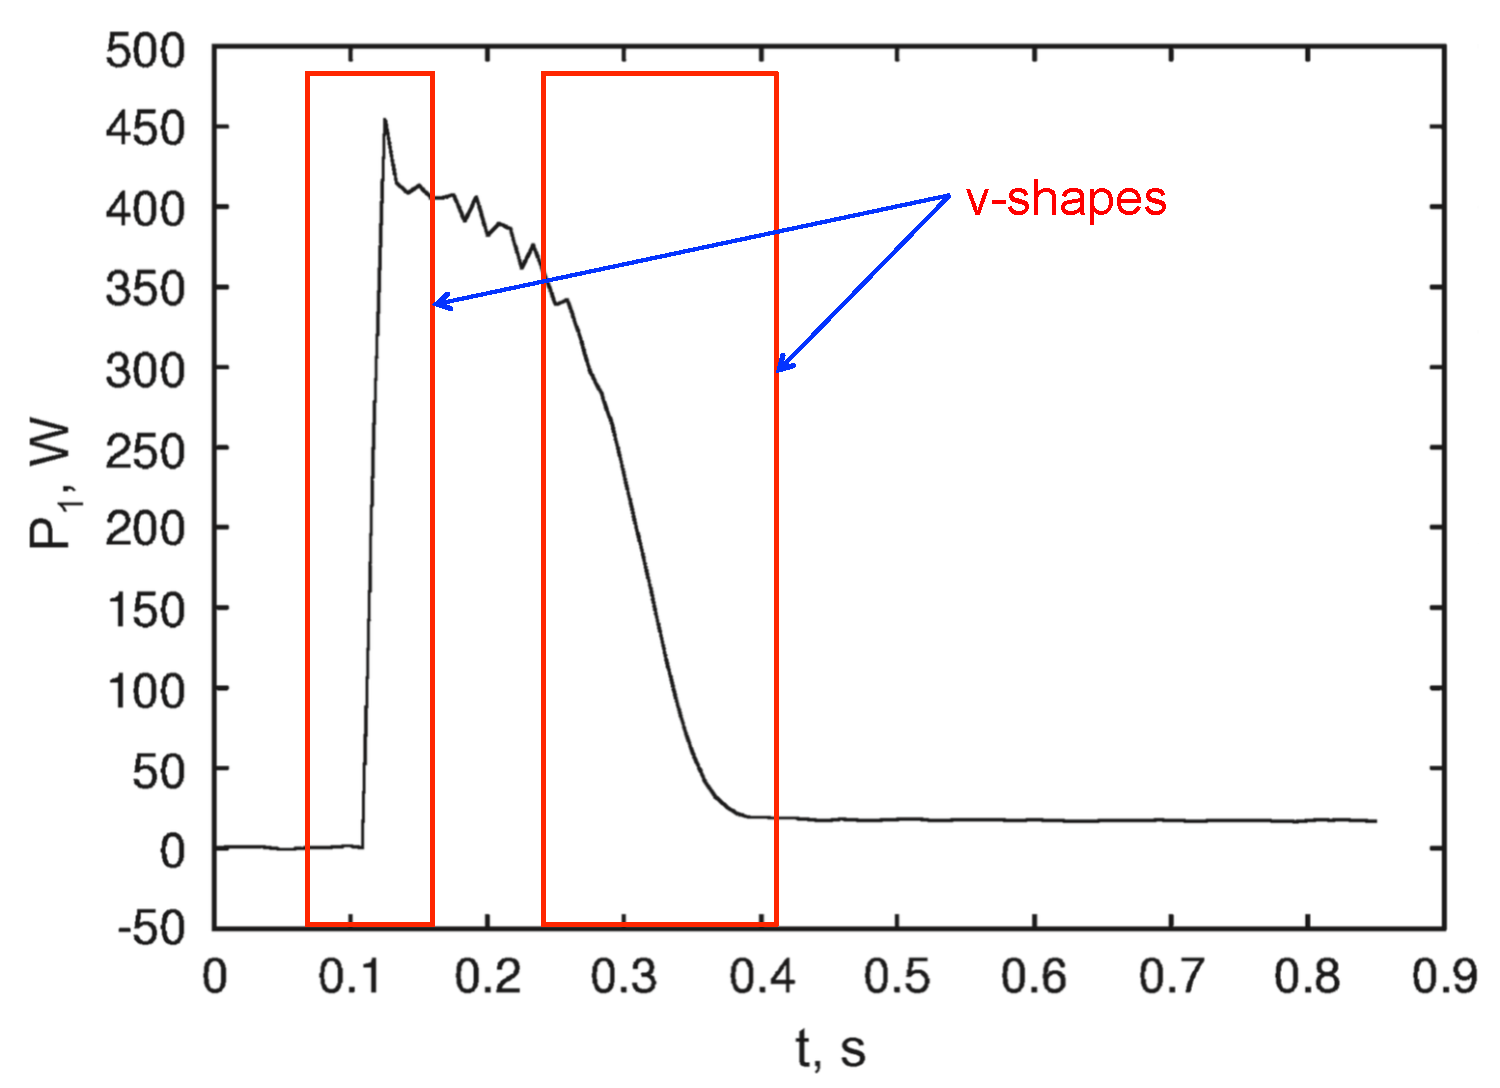
\includegraphics[width=0.6\textwidth]{./chapters/chapter2/images/v-shape.pdf} 
\caption{\textit{v-shapes} on the transient of an induction motor~\cite{Leeb95PD}.} 
\label{fig:A15} 
\end{figure}


A limitation of the transient-based algorithms relates to the simultaneous operation in which two or more devices are switched on at the same time. To overcome this restriction, in~\cite{Srinivasan06PD}, Fast Fourier Transform (FFT) is applied to analyze the harmonics of the incoming current waveform. Both real and imaginary parts of the harmonics are the inputs of an ANN, in which the number of inputs depends on the effectiveness of the additional harmonics, while the number of outputs relates to the number of classes, i.e. number of known devices. Figure~\ref{fig:A16} represents the mean value and standard deviation of the harmonics of some typical devices.
\begin{figure}
\centering
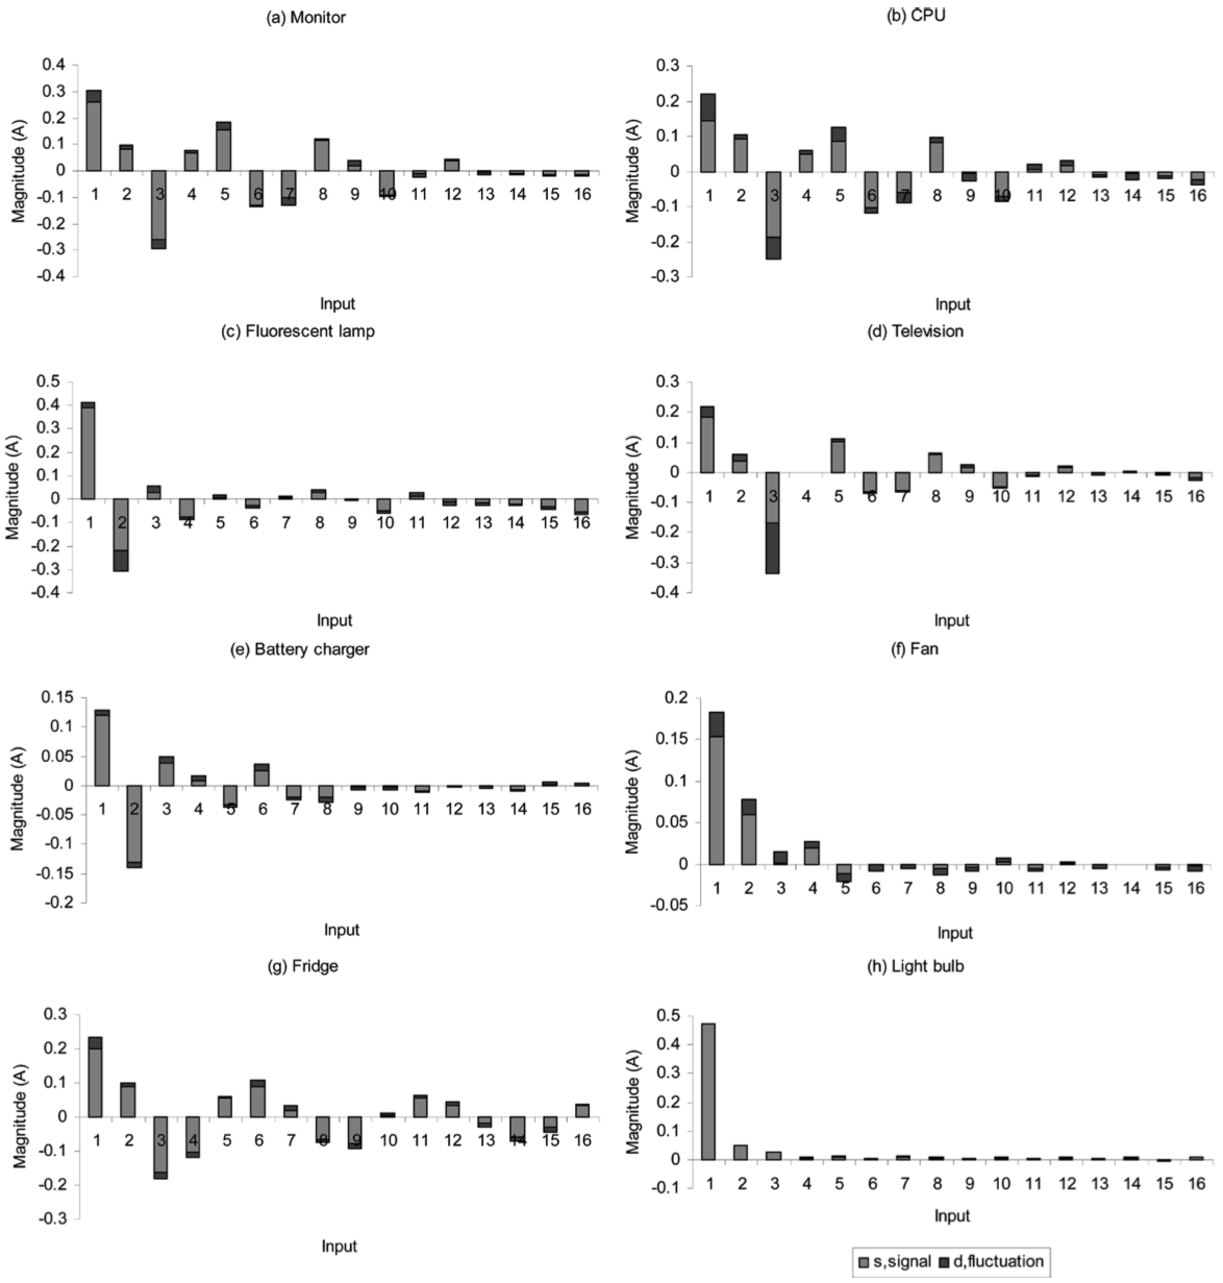
\includegraphics[width=1\textwidth]{./chapters/chapter2/images/harmonic_of_devices.pdf} 
\caption{Harmonic signatures of typical devices~\cite{Srinivasan06PD}.} 
\label{fig:A16} 
\end{figure}

Besides analyzing the spectral and harmonic content, a novel method using V-I trajectory to categorize the groups of devices is also proposed in \cite{Lee04,Lam07}. The V-I trajectory is plotted for each device using the normalized current and voltage values. Figure~\ref{fig:A17} illustrates an example of the voltage and current waveforms of a television and the corresponding V-I trajectory. This method can form a high performance due to the distinctive V-I curves of devices. However, it is sensitive to the operation scenario of the multi-state loads. Moreover, the trajectory patterns of small loads are difficult to be distinguished.

\begin{figure}
\centering
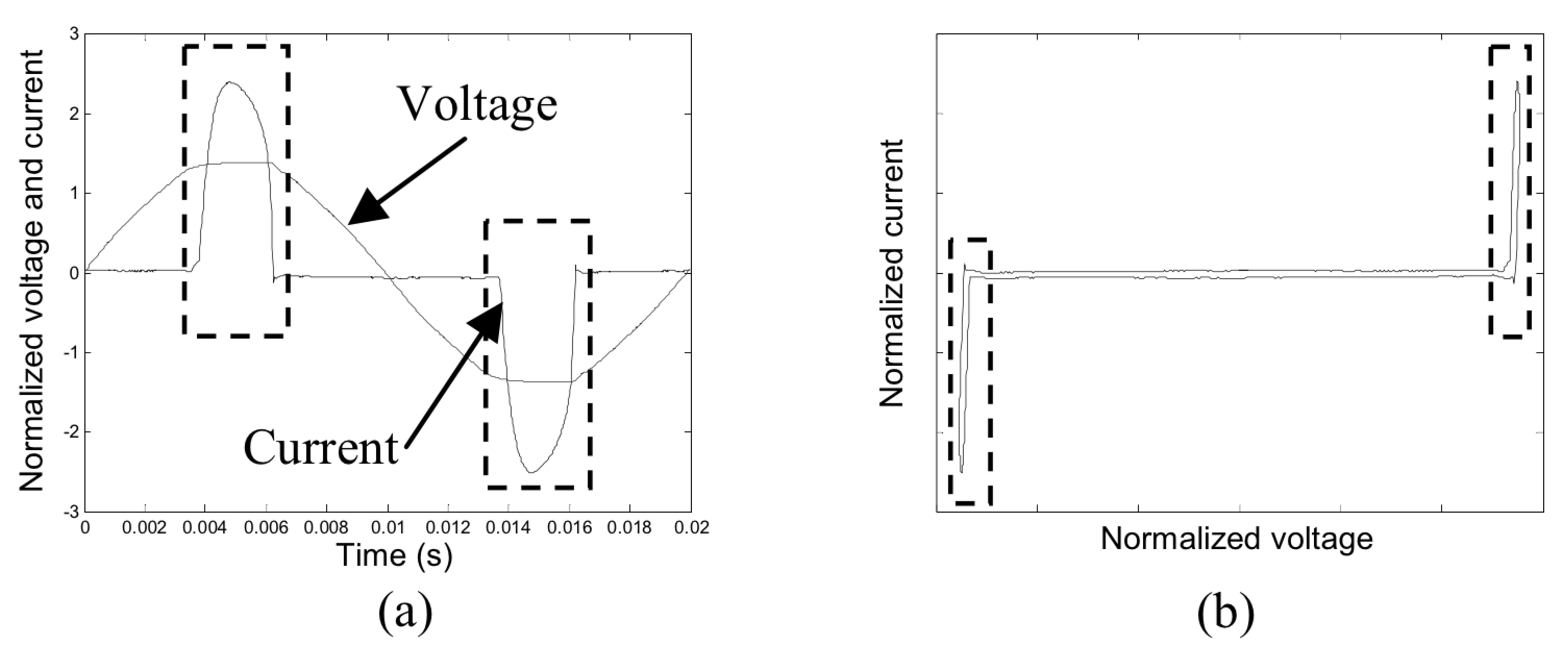
\includegraphics[width=0.9\textwidth]{./chapters/chapter2/images/VItrajectory.pdf} 
\caption{(a) Current and voltage waveforms of a television. (b) Corresponding V-I trajectory~\cite{Lam07}.} 
\label{fig:A17} 
\end{figure}

In another research, the authors of~\cite{Gupta10} introduce a new approach to identify the running devices by detecting the noise created on the monitored power line, based on a high frequency hardware and 2048-point FFT. In homes and buildings, there are some devices running on background and their power waveform is detected and saved on the memory. Whenever a new device is turned on, a noise is created on the background and the respective new device can be identified by analyzing the frequency components of the measured signal. For example, Figure~\ref{fig:A18} shows the new signal appearing on the background noise and its extracted frequency components. 
\begin{figure}
\centering
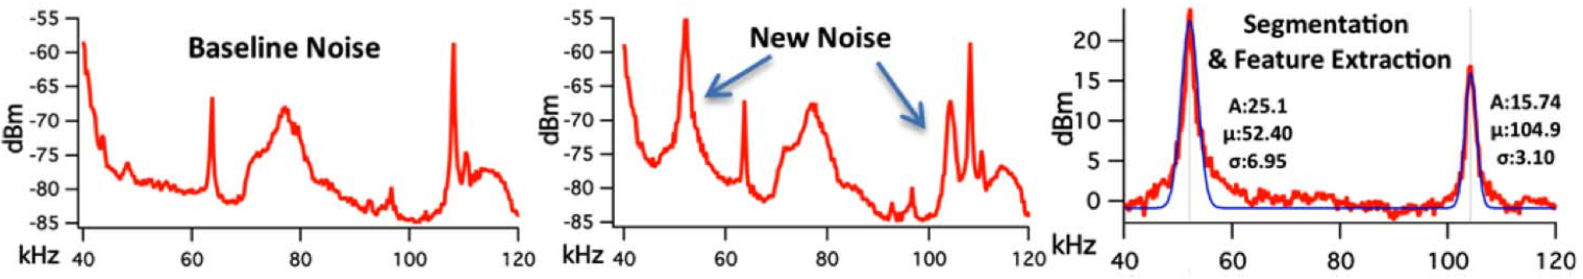
\includegraphics[width=1\textwidth]{./chapters/chapter2/images/noiseEMI.pdf} 
\caption{New noise feature extracted from the background noise~\cite{Gupta10}.} 
\label{fig:A18} 
\end{figure}

Similarly, a system called Detecting Operating States of Electronic devices (DOSE)~\cite{Chen15} tries to detect the variation on the electromagnetic field to identify the corresponding devices. The Electromagnetic Interference (EMI), generated when an electronic device operates, is coupled to the power line and its form is picked up by a sensing hardware attached to the outlet. As shown in Figure~\ref{fig:A19}, the time-varying EMI of a laptop is different and distinguishable at idle, medium load and high load.

\begin{figure}
\centering
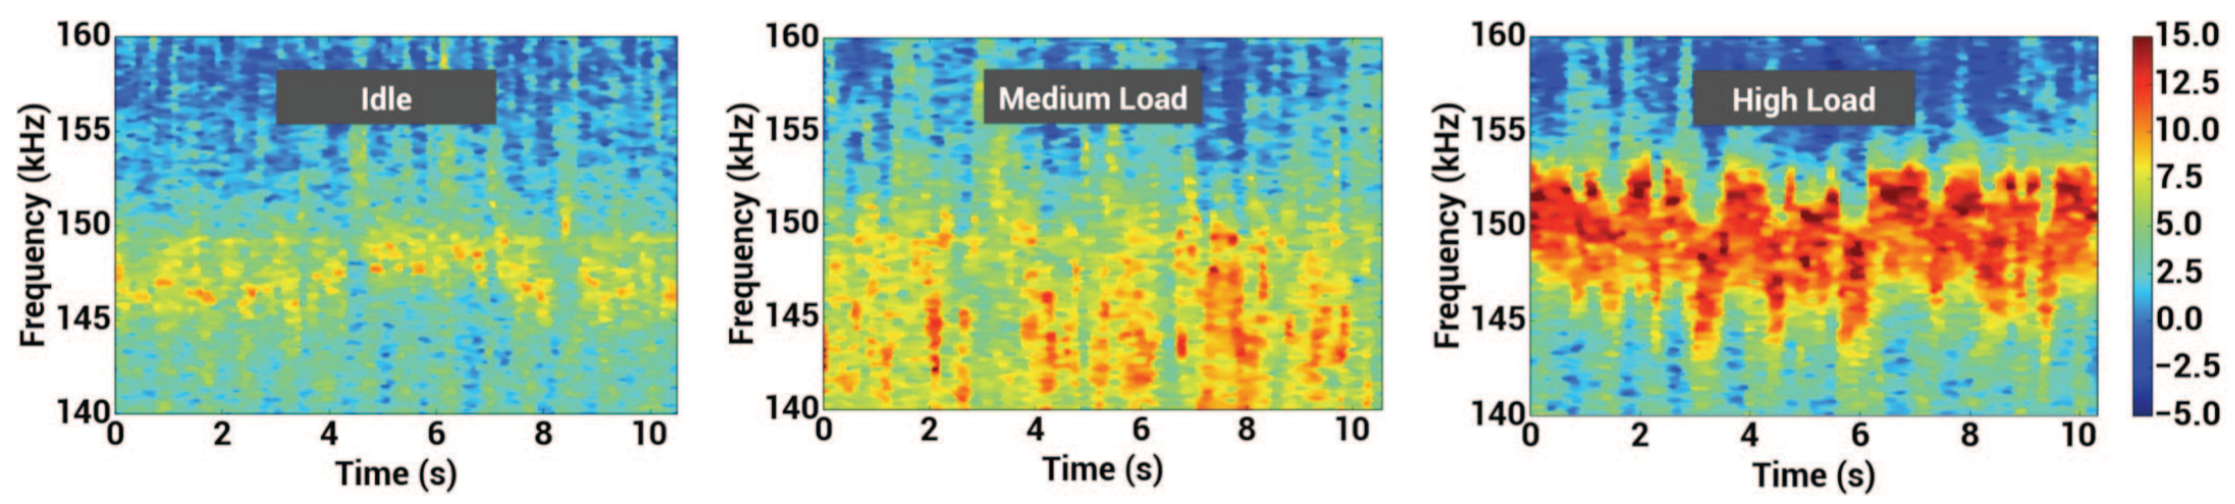
\includegraphics[width=1\textwidth]{./chapters/chapter2/images/DOSE.pdf} 
\caption{Time-varying EMI of a laptop at idle, medium load and high load~\cite{Chen15}.} 
\label{fig:A19} 
\end{figure}
Although high-frequency based methods show a perspective to significantly improve device identification, the most important drawback preventing it from being widely implemented is the deployment cost, which increases along with the frequency of hardware.